\chapter{Vergleich der Browser}
\label{chapter:vergleich-der-browser}

- Zusammenfassung: Vergleich Tor v. Firefox und Brave v. Chrome

\subsection*{Common Locations}
- Process Monitor Logfiles: 
	> Keine PB Artefakte bei beiden Browsern
	> Abbildung Anzahl Schreiboperationen pro Browser
- SQLite Datenbänke
	> Keine PB Artefakte in SQLite Datenbänken beider Browser
	> Gleiche Datenbänke: Evtl. hervorheben, bei welchen Browser mehr geschrieben wurde, ODER: Diagramm mit Anazhl Schreiboperationen pro SQLite DB verglichen zwischen Browsern
		(Gestacktes Balkendiagramm zu veränderten SQLite DBs => Erst bei Vergleich mit Tor!)

\subsection*{Uncommon Locations}
- Autopsy Stichwortsuche: keine Suchergebnisse bei beiden Browsern
- Autopsy Kategorien: keine PB Artefakten in kategorisierten Dateien, evtl. unterschiedlich Kategorisierte Dateien hervorheben
- Volatility Artefakte:




\paragraph*{Firefox Zusammenfassung Yarascan}
Wie in Abbildung \ref{chart:firefox-volatility-summary} zusammenfassend gezeigt wurden vor dem Browsing Szenario, keine private Browsing Artefakte im ersten RAM Dump gefunden.
Nach dem Browsing Szenario mit geöffnetem Browser konnten die meisten Artefakte identifiziert werden. Dabei wurden am häufigsten URL Artefakte in Firefox Prozessen gefunden. Zudem konnte hier das E-Mail Passwort im Klartext lokalisiert werden.
Nach Schließen des Browsers konnten im dritten Snapshots URLs im DNSCache Windows Service gefunden werden. Nach leeren des Caches und Beenden des DNSCache Services konnten wurden keine Artefakte gefunden.
\begin{table}[h!]
	\resizebox{\linewidth}{!}{
	\begin{tabular}{r}
		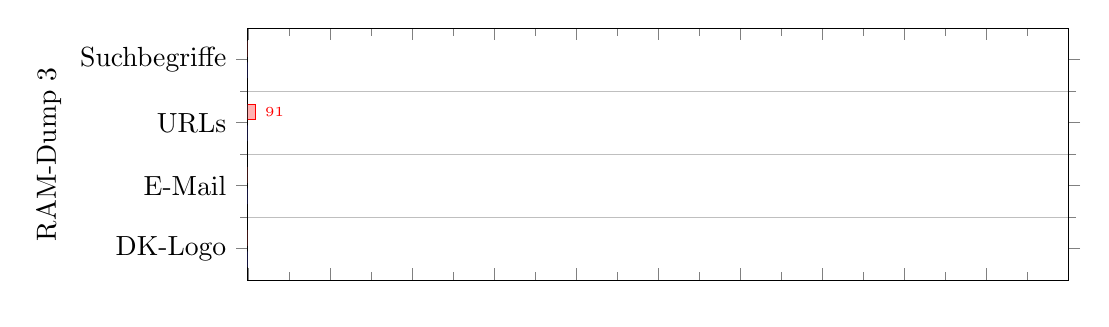
\begin{tikzpicture}
			\begin{axis}[
			xbar,
			width=12cm, 
			height=3cm, 
			ylabel style={align=center}, ylabel=RAM-Dump 3,
			y=0.8cm,
			symbolic y coords={DK-Logo, E-Mail, URLs, Suchbegriffe},
			ytick=data,
			xticklabels={,,},
            xmin = 0,
            xmax = 10000,
			nodes near coords, 
			nodes near coords align={horizontal},
			nodes near coords style={font=\tiny},
   			nodes near coords={\pgfmathfloatifflags{\pgfplotspointmeta}{0}{}{\pgfmathprintnumber{\pgfplotspointmeta}}},
			bar width=.2cm,
			enlarge y limits={abs=2*\pgfplotbarwidth},
			scaled x ticks=false,
    		yminorgrids = true,minor tick num=1
			]
				\addplot coordinates {
				(0,DK-Logo) (0,E-Mail) (0,URLs) (0,Suchbegriffe)
				};
				\addplot coordinates {
				(0,DK-Logo) (0,E-Mail) (91,URLs) (0,Suchbegriffe)
				};
			\end{axis}
		\end{tikzpicture}
		\\
		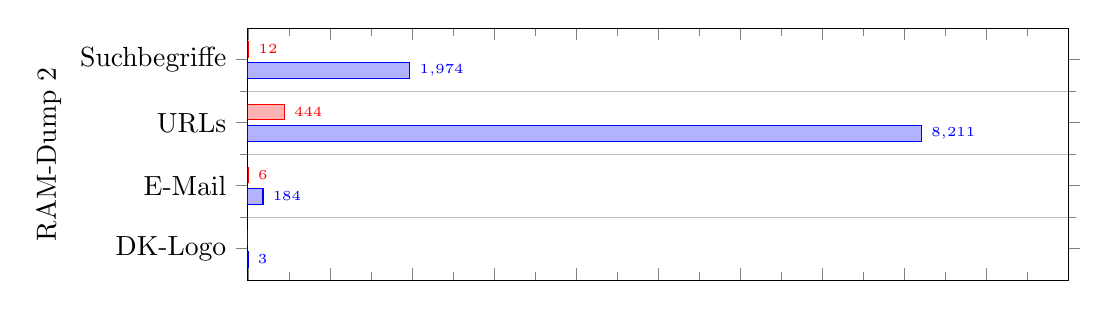
\begin{tikzpicture}
			\begin{axis}[
			xbar,
			width=12cm, 
			height=3cm, 
			ylabel style={align=center}, ylabel=RAM-Dump 2,
			y=0.8cm,
			symbolic y coords={DK-Logo, E-Mail, URLs, Suchbegriffe},
			ytick=data,
			xticklabels={,,},
            xmin = 0,
            xmax = 10000,
			nodes near coords, 
			nodes near coords align={horizontal},
			nodes near coords style={font=\tiny},
   			nodes near coords={\pgfmathfloatifflags{\pgfplotspointmeta}{0}{}{\pgfmathprintnumber{\pgfplotspointmeta}}},
			bar width=.2cm,
			enlarge y limits={abs=2*\pgfplotbarwidth},
			scaled x ticks=false,
    		yminorgrids = true,minor tick num=1
			]
				\addplot coordinates {
				(3,DK-Logo) (184,E-Mail) (8211,URLs) (1974,Suchbegriffe)
				};
				\addplot coordinates {
				(0,DK-Logo) (6,E-Mail) (444,URLs) (12,Suchbegriffe)
				};
			\end{axis}
		\end{tikzpicture}
		\\
		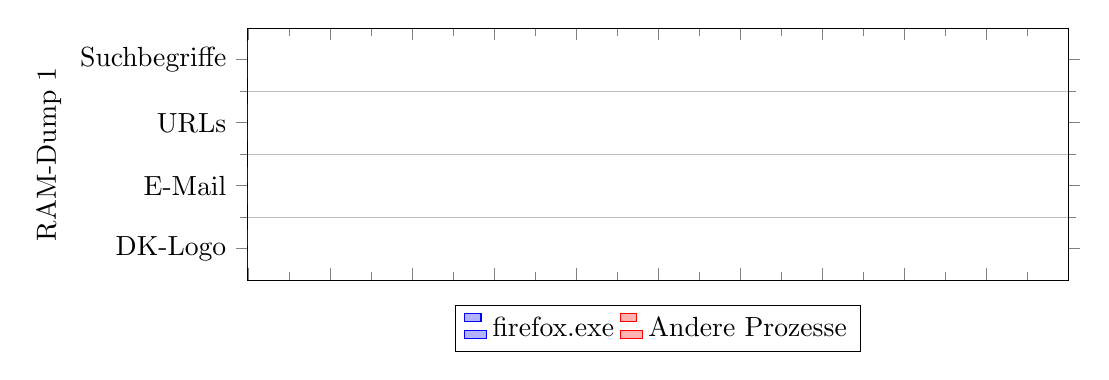
\begin{tikzpicture}
			\begin{axis}[
			xbar,
			width=12cm, 
			height=3cm, 
			ylabel style={align=center}, ylabel=RAM-Dump 1,
			y=0.8cm,
			symbolic y coords={DK-Logo, E-Mail, URLs, Suchbegriffe},
			ytick=data,
			xticklabels={,,},
            xmin = 0,
            xmax = 10000,
			nodes near coords, 
			nodes near coords align={horizontal},
			nodes near coords style={font=\small},
   			nodes near coords={\pgfmathfloatifflags{\pgfplotspointmeta}{0}{}{\pgfmathprintnumber{\pgfplotspointmeta}}},
			bar width=.2cm,
			enlarge y limits={abs=2*\pgfplotbarwidth},
			legend style={
				at={(0.5,-0.1)},
				anchor=north
			},
			legend columns=2,
			scaled x ticks=false,
    		yminorgrids = true,minor tick num=1
			]
			\addplot coordinates {
			(0,DK-Logo) (0,E-Mail) (0,URLs) (0,Suchbegriffe)
			};
			\addplot coordinates {
			(0,DK-Logo) (0,E-Mail) (0,URLs) (0,Suchbegriffe)
			};
			\legend{firefox.exe, Andere Prozesse}
			\end{axis}
		\end{tikzpicture}	
	\end{tabular}
	}
	\caption{Zusammenfassung gefundener Artefakte in den Firefox RAM-Dumps}
	\label{chart:firefox-volatility-summary}
\end{table}






\paragraph*{Tor: Zusammenfassung Yarascan}
Wie in Abbildung \ref{chart:tor-volatility-summary} zusammenfassend gezeigt, wurden ausschließlich nach dem Browsing-Szenario vor (RAM-Dump 2) und nach (RAM-Dump 3-1) Zuweisung einer "Neuen Identität" Brwosing Artefakte im Arbeitsspeicher gefunden.
Nach dem Browsing Szenario mit geöffnetem Browser konnten die meisten Artefakte identifiziert werden. Dabei wurden am häufigsten URL Artefakte in Firefox Prozessen gefunden. Zudem konnte hier das E-Mail Passwort im Klartext lokalisiert werden.
Nach Schließen des Browsers konnten im dritten Snapshots URLs im DNSCache Windows Service gefunden werden. Nach leeren des Caches und Beenden des DNSCache Services konnten wurden keine Artefakte gefunden.
Die Erstellung einer "Neuen Identität" reduzierte dabei deutlich die gefundenen Artefakte im RAM.
In keinem RAM-Speicherabbild konnten HTML-Fragmente der im Browsing-Szenario besuchten Seiten identifiziert werden. Weiterhin wurde zwei Mal das Passwort des Google-Accounts im Klartext gefunden.

\begin{table}[h!]
	\renewcommand{\arraystretch}{0.4}
	\resizebox{\linewidth}{!}{
	\begin{tabular}{r}
		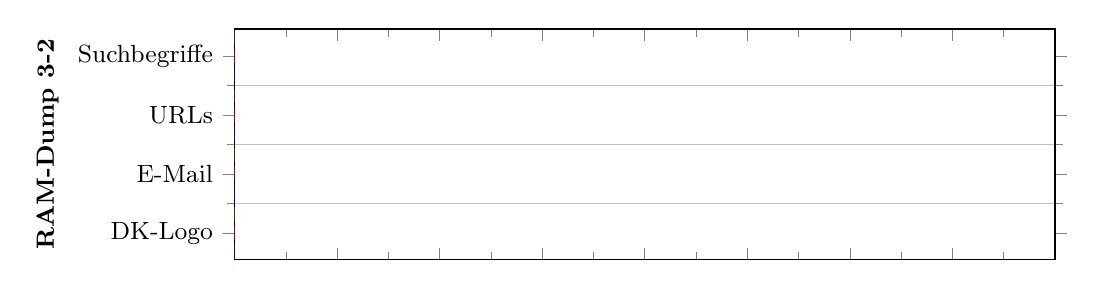
\begin{tikzpicture}
			\begin{axis}[
			xbar,
			width=12cm, 
			height=3cm, 
			ylabel style={align=center}, ylabel=\textbf{RAM-Dump 3-2},
			y=0.75cm,
			symbolic y coords={DK-Logo, E-Mail, URLs, Suchbegriffe},
			label style={font=\small},
			tick label style={font=\small},
			ytick=data,
			xticklabels={,,},
            xmin = 0,
            xmax = 40000,
			nodes near coords, 
			nodes near coords align={horizontal},
			nodes near coords style={font=\tiny},
   			nodes near coords={\pgfmathfloatifflags{\pgfplotspointmeta}{0}{}{\pgfmathprintnumber{\pgfplotspointmeta}}},
			bar width=.17cm,
			enlarge y limits={abs=2*\pgfplotbarwidth},
			scaled x ticks=false,
			legend style={
				at={(0.5,-0.1)},
				anchor=north
			},
			legend columns=3,
    		yminorgrids = true,minor tick num=1
			]
				\addplot coordinates {
				(0,DK-Logo) (0,E-Mail) (0,URLs) (0,Suchbegriffe)
				};
				\addplot coordinates {
				(0,DK-Logo) (0,E-Mail) (0,URLs) (0,Suchbegriffe)
				};
								\addplot coordinates {
				(0,DK-Logo) (0,E-Mail) (0,URLs) (0,Suchbegriffe)
				};
			\end{axis}
		\end{tikzpicture}
		\\[-7pt]
		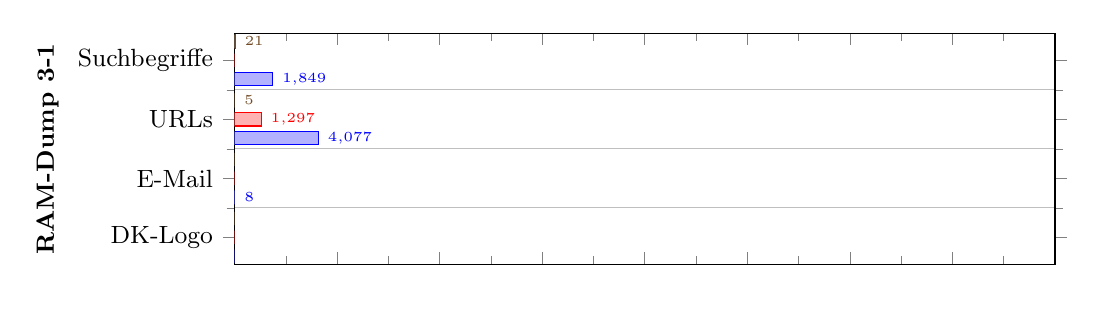
\begin{tikzpicture}
			\begin{axis}[
			xbar,
			width=12cm, 
			height=3cm, 
			ylabel style={align=center}, ylabel=\textbf{RAM-Dump 3-1},
			y=0.75cm,
			symbolic y coords={DK-Logo, E-Mail, URLs, Suchbegriffe},
			label style={font=\small},
			tick label style={font=\small},
			ytick=data,
			xticklabels={,,},
            xmin = 0,
            xmax = 40000,
			nodes near coords, 
			nodes near coords align={horizontal},
			nodes near coords style={font=\tiny},
   			nodes near coords={\pgfmathfloatifflags{\pgfplotspointmeta}{0}{}{\pgfmathprintnumber{\pgfplotspointmeta}}},
			bar width=.17cm,
			enlarge y limits={abs=2*\pgfplotbarwidth},
			scaled x ticks=false,
			legend style={
				at={(0.5,-0.1)},
				anchor=north
			},
			legend columns=3,
    		yminorgrids = true,minor tick num=1
			]
				\addplot coordinates {
				(0,DK-Logo) (8,E-Mail) (4077,URLs) (1849,Suchbegriffe)
				};
				\addplot coordinates {
				(0,DK-Logo) (0,E-Mail) (1297,URLs) (0,Suchbegriffe)
				};
				\addplot coordinates {
				(0,DK-Logo) (0,E-Mail) (5,URLs) (21,Suchbegriffe)
				};
			\end{axis}
		\end{tikzpicture}
		\\[-7pt]
		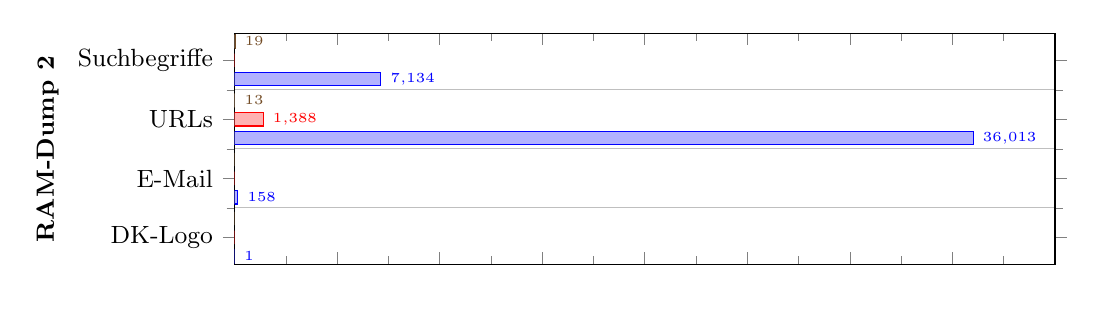
\begin{tikzpicture}
			\begin{axis}[
			xbar,
			width=12cm, 
			height=3cm, 
			ylabel style={align=center}, ylabel=\textbf{RAM-Dump 2},
			y=0.75cm,
			symbolic y coords={DK-Logo, E-Mail, URLs, Suchbegriffe},
			label style={font=\small},
			tick label style={font=\small},
			ytick=data,
			xticklabels={,,},
            xmin = 0,
            xmax = 40000,
			nodes near coords, 
			nodes near coords align={horizontal},
			nodes near coords style={font=\tiny},
   			nodes near coords={\pgfmathfloatifflags{\pgfplotspointmeta}{0}{}{\pgfmathprintnumber{\pgfplotspointmeta}}},
			bar width=.17cm,
			enlarge y limits={abs=2*\pgfplotbarwidth},
			scaled x ticks=false,
			legend style={
				at={(0.5,-0.1)},
				anchor=north
			},
			legend columns=3,
    		yminorgrids = true,minor tick num=1
			]
				\addplot coordinates {
				(1,DK-Logo) (158,E-Mail) (36013,URLs) (7134,Suchbegriffe)
				};
				\addplot coordinates {
				(0,DK-Logo) (0,E-Mail) (1388,URLs) (0,Suchbegriffe)
				};
				\addplot coordinates {
				(0,DK-Logo) (0,E-Mail) (13,URLs) (19,Suchbegriffe)
				};
			\end{axis}
		\end{tikzpicture}
		\\[-7pt]
		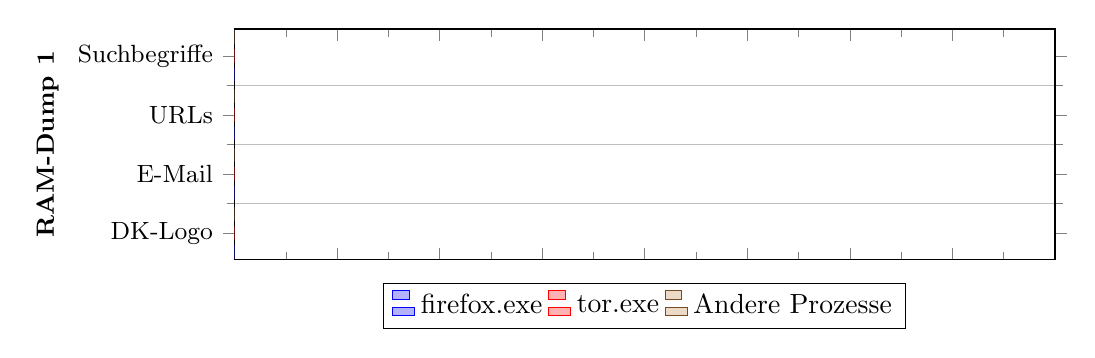
\begin{tikzpicture}
			\begin{axis}[
			xbar,
			width=12cm, 
			height=3cm, 
			ylabel style={align=center}, ylabel=\textbf{RAM-Dump 1},
			y=0.75cm,
			symbolic y coords={DK-Logo, E-Mail, URLs, Suchbegriffe},
			label style={font=\small},
			tick label style={font=\small},
			ytick=data,
			xticklabels={,,},
            xmin = 0,
            xmax = 40000,
			nodes near coords, 
			nodes near coords align={horizontal},
			nodes near coords style={font=\tiny},
   			nodes near coords={\pgfmathfloatifflags{\pgfplotspointmeta}{0}{}{\pgfmathprintnumber{\pgfplotspointmeta}}},
			bar width=.17cm,
			enlarge y limits={abs=2*\pgfplotbarwidth},
			scaled x ticks=false,
			legend style={
				at={(0.5,-0.1)},
				anchor=north
			},
			legend columns=3,
    		yminorgrids = true,minor tick num=1
			]
			\addplot coordinates {
			(0,DK-Logo) (0,E-Mail) (0,URLs) (0,Suchbegriffe)
			};
			\addplot coordinates {
			(0,DK-Logo) (0,E-Mail) (0,URLs) (0,Suchbegriffe)
			};
						\addplot coordinates {
			(0,DK-Logo) (0,E-Mail) (0,URLs) (0,Suchbegriffe)
			};
			\legend{firefox.exe, tor.exe, Andere Prozesse}
			\end{axis}
		\end{tikzpicture}	
	\end{tabular}
	}
	\caption{Zusammenfassung gefundener Artefakte in den Tor-Browser RAM-Dumps}
	\label{chart:tor-volatility-summary}
\end{table}















\subsection*{Registry}


	
 "Sessionstore-Backup" fehlt in Tor

TODO: Kreisdiagramme/Balkendiagramme mit Gesamtzahl an (Non-)Firefox Yarascan-Treffer erst im Vergleich mit Tor
- Firefox v. Chrome ("Standardbrowser")
- Tor v. Brave ("Sichere Browser")
- Zum Schluss: "Eine große Tabelle" mit den wichtigsten Kategorien?